We started out by assessing the skills of each team member and breaking down the task into smaller sub tasks.  We then made an initial allocation of team members to sub tasks based on our assessment of matching skills to the tasks.

On a day-to-day basis we tracked the progress of the project by using an online task and project management web system called Agilefant. 

Agilefant allows one to set up projects, assign team members, break the project down into major tasks and split the tasks down into smaller sub tasks and set up dependencies between the small tasks.

In our case we broke the software down into “core”, “client” and “services” and initially allocated at most two team members to each section.  As time progressed, based on how quickly we were getting different sections done and depending on if there were dependencies which needed to be worked on, we moved people around and reallocated tasks.


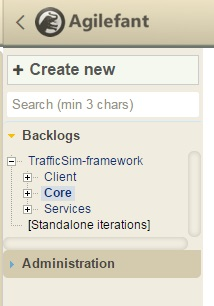
\includegraphics[scale=0.7]{./images/menu.jpg}

Agilefant allowed us to see at a glance how the small tasks within each of the major subtasks was going and how we were progressing towards our target.  It also alerted us to any dependencies which needed doing urgently and helped us make decisions about moving team members onto different tasks. \\
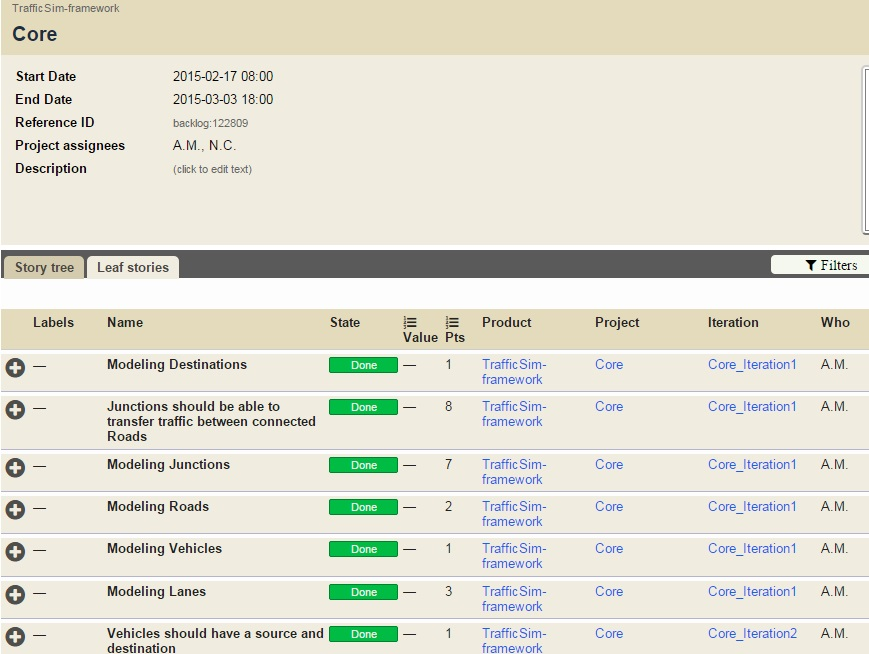
\includegraphics[scale=0.5]{./images/tasks.jpg}

The “burnup” chart shows completed tasks in green against the total scope of the sub-project. 
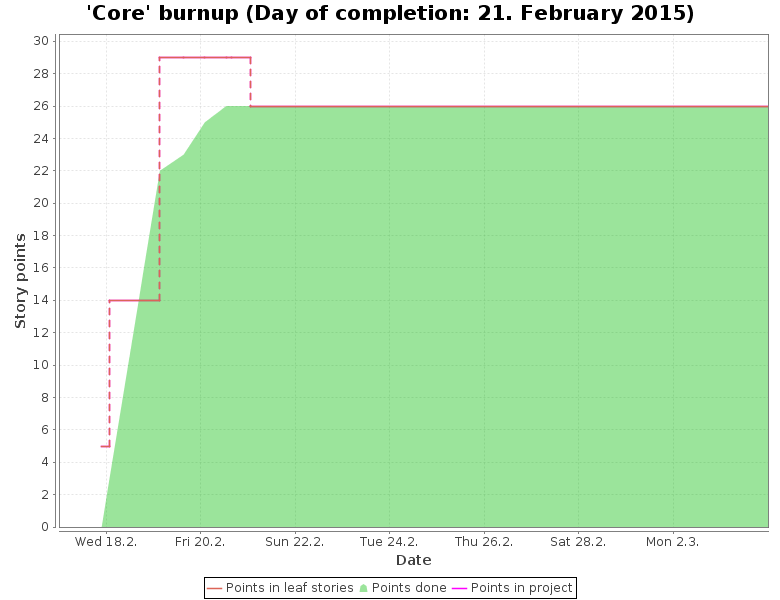
\includegraphics[scale=0.3]{./images/burnup_chart.png}

Dependencies can be clearly identified \\
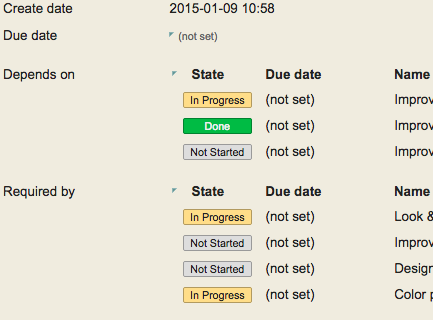
\includegraphics[]{./images/dependencies.png}

The sub-teams for the sub-projects core, client and services each consisted of one or more team member(s) at any one time.  There was overlap as any team member might be in more than one sub-team at any one time.  We allocated one person to be the team leader for each sub team at any one time.  The team leader was responsible for allocating tasks within the sub-team and also for identifying any problems and dependencies.  The sub-teams worked independently from each other and could organise their own meetings or ways of working as they saw fit.

We had weekly whole team progress meetings to evaluate how each sub-team was performing and discuss any necessary changes to the overall structure of the group or of the project. The team leaders for each sub-team reported to the whole group and made recommendations about resourcing which were discussed and agreed upon at the meeting. Any changes agreed were recorded and subsequently emailed to all team members. These meetings were also intended to be used for any conflict resolution, with group consensus determining the outcome of any disagreements, however in practice there were very few disagreements and none that could not be resolved before reaching this point. We also maintained a group on an instant messaging service which was used to communicate key pieces of information to each other and update each other on important developments.

Our team organisation and dynamic allowed us to maintain progress throughout the project timeframe, and we were well equipped to deal with one member falling behind due to impairment, however we did not anticipate two members becoming impaired at the same time as was unfortunately the case when two members suffered bereavements within a short timeframe of one another which slowed down our overall progress.